\documentclass{article}
\usepackage{graphicx}
\usepackage[utf8]{inputenc}
\usepackage{amsmath, amssymb, latexsym}
\usepackage{neuralnetwork}
\usepackage{multicol}

\usepackage{pgfplots}
\usepackage{algorithm}
\usepackage[noend]{algpseudocode}
\usepackage{tikz}
\usepackage{nicefrac}
\pgfplotsset{every axis legend/.append style={
at={(0,0)},
anchor=north east}}
\usetikzlibrary{shapes,positioning,intersections,quotes}
\usetikzlibrary{arrows.meta,
                bending,
                intersections,
                quotes,
                shapes.geometric}
                
\definecolor{darkgreen}{rgb}{0.0, 0.6, 0.0}
\definecolor{darkred}{rgb}{0.7, 0.0, 0.0}
\makeatletter
\def\BState{\State\hskip-\ALG@thistlm}
\makeatother
\title{Week 9}
\begin{document}
\pagenumbering{gobble}
\maketitle
\newpage
\pagenumbering{arabic}

\section*{Types of classification problems with NNs}
\begin{itemize}
  \item Training set is ${(x^1, y^1), (x^2, y^2), ..., (x^n, y^n)}$.
  \item $L$ = number of layers in the network.
  \item $s_l$ = number of units (not counting bias unit) in layer $l$.
\end{itemize}

\begin{neuralnetwork}[height=6]
  \newcommand{\x}[2]{$x_#2$}
  \newcommand{\hfirst}[2]{\small $a^{(1)}_#2$}
  \newcommand{\hsecond}[2]{\small $a^{(2)}_#2$}
  \newcommand{\hthird}[2]{\small $a^{(3)}_#2$}
  \inputlayer[count=3, bias=true, title=Input\\layer, text=\x]
  \hiddenlayer[count=5, bias=true, title=Hidden\\layer, text=\hfirst] \linklayers\\
  \hiddenlayer[count=5, bias=true, title=Hidden\\layer, text=\hsecond] \linklayers
  \hiddenlayer[count=4, bias=false, title=Hidden\\layer, text=\hthird] \linklayers
\end{neuralnetwork}

~\\
So here we have:
\begin{itemize}
  \item $L=4$.
  \item $s_1 = 3$.
  \item $s_2 = 5$.
  \item $s_3 = 5$.
  \item $s_4 = 4$.
\end{itemize}

\subsection*{Binary classification}
\begin{itemize}
  \item 1 output (0 or 1).
  \item So single output node - value is going to be a real number.
  \item $k = 1$.
  \item $s_l = 1$
\end{itemize}

\subsection*{Multi-class classification}
\begin{itemize}
  \item $k$ distinct classifications.
  \item $y$ is a $k$-dimensional vector of real numbers.
  \item $s_l = k$
\end{itemize}

\section*{Cost function}

Logistic regression cost function is as follows:

$$J(\theta) = -\frac{1}{m} [\sum_{i=1}^{m} y^{(i)} log h_{\theta}(x^{(i)}) + (1- y^{(i)})log(1 - h_{\theta}(x^{(i)}))] +  \frac{\lambda}{2m} \sum_{j=1}^{m} \theta_j^2$$


~\\
For neural networks our cost function is a generalization of this equation above, so instead of one output we generate $k$ outputs:

$$J(\Theta) = -\frac{1}{m} [\sum_{i=1}^{m} \sum_{k=1}^{K} y^{(i)}_k log (h_{\Theta}(x^{(i)}))_k + (1- y^{(i)}_k)log(1 - (h_{\Theta}(x^{(i)}))_k)] +  \frac{\lambda}{2m} \sum_{l=1}^{L-1} \sum_{i=1}^{s_l} \sum_{j=1}^{s_l+1} (\Theta^{(l)}_{ji})^2$$

~\
\begin{itemize}
  \item Our cost function now outputs a $k$ dimensional vector.
  \item Costfunction $J(\Theta)$ is $-1/m$ times a sum of a similar term to which we had for logic regression.
  \item But now this is also a sum from $k = 1$ through to $K$ ($K$ is number of output nodes).
  \item Summation is a sum over the $k$ output units - i.e. for each of the possible classes.
  \item We don't sum over the bias terms (hence starting at 1 for the summation).
\end{itemize}

\subsection*{Partial derivative terms}

\begin{itemize}
  \item $\Theta^{(1)}$ is the matrix of weights which define the function mapping from layer 1 to layer 2.
  \item $\Theta^{(1)}_{10}$  is the real number parameter which you multiply the bias unit (i.e. 1) with for the bias unit input into the first unit in the second layer.
  \item $\Theta^{(1)}_{11}$ is the real number parameter which you multiply the first (real) unit with for the first input into the first unit in the second layer.
  \item $\Theta^{(1)}_{21}$  is the real number parameter which you multiply the first (real) unit with for the first input into the second unit in the second layer.
\end{itemize}

\subsection*{Gradient computation}

\begin{itemize}
  \item One training example.
  \item Imagine we just have a single pair (x,y) - entire training set.
  \item The following is how the forward propagation method works:
  \item Layer 1: $a^{(1)} = x$ and $z^{(2)} = \Theta^{(1)}a^{(1)}$.
  \item Layer 2: $a^{(2)} = g(z^{(2)}) + a^{(2)}_0$ and $z^{(3)} = \Theta^{(2)}a^{(2)}$.
  \item Layer 3: $a^{(3)} = g(z^{(3)}) + a^{(3)}_0$ and $z^{(4)} = \Theta^{(3)}a^{(3)}$.
  \item Ouptut: $a^{(4)} = h_{\Theta}(x) = g(z^{(4)})$.

\end{itemize}

\begin{neuralnetwork}[height=5]
  \newcommand{\x}[2]{$x_#2$}
  \newcommand{\hfirst}[2]{\small $a^{(1)}_#2$}
  \newcommand{\hsecond}[2]{\small $a^{(2)}_#2$}
  \newcommand{\hthird}[2]{\small $a^{(3)}_#2$}
  \newcommand{\hforth}[2]{\small $a^{(4)}_#2$}
  \hiddenlayer[count=4, bias=true, title=Layer 1, text=\hfirst] \linklayers\\
  \hiddenlayer[count=4, bias=true, title=Layer 2, text=\hsecond] \linklayers
  \hiddenlayer[count=4, bias=true, title=Layer 3, text=\hthird] \linklayers
  \hiddenlayer[count=4, bias=false, title=Layer 4, text=\hforth] \linklayers
\end{neuralnetwork}

\subsection*{Calculate backpropagation}

\begin{itemize}
  \item $\delta_j$ is $Lx1$ vector.
  \item First we compute the LAST element: $\delta^{(L)}_j = a^{(L)}_j - y_j$.
  \item Value of each element is based on the value of the next element:

        $$\delta^{(l)}_j = (\Theta^{(l)}_j)^T\delta^{(l+1)}_j \cdot g'(z^{(l)}_j)$$

  \item Finally, use $\Delta$ to accumulate the partial derivative terms:

        $$\Delta^{(l)}_{ij} := \Delta^{(l)}_{ij} + a^{(l)}_j\delta^{(l+1)}_i$$

  \item $l$ = layer.
  \item $j$ = node in that layer.
  \item $i$ = the error of the affected node in the target layer

\end{itemize}


\begin{equation*}
\Large
\frac{\partial}{\partial \Theta^{(l)}_{ij}}J(\Theta) = \begin{cases}
          \frac{1}{m} \Delta^{(l)}_{ij} + \lambda \Theta ^{(l)}_{ij} \quad &\text{if} \, j \neq 0 \\
          \frac{1}{m} \Delta^{(l)}_{ij} \quad &\text{if} \, j=0 \\
     \end{cases}
\end{equation*}

\subsection*{Gradient checking}

Backpropagation contains a lot of details, and tiny flaws can break it.
As a result, employing a numerical approach to verify the gradient can aid in the quick diagnosis of a problem.

\begin{itemize}
  \item Have a function $J(\Theta)$.
  \item Compute $\Theta + \epsilon$.
  \item Compute $\Theta - \epsilon$.
  \item Join them by a straight line.
  \item Use the slope of that line as an approximation to the derivative.
\end{itemize}

~\\
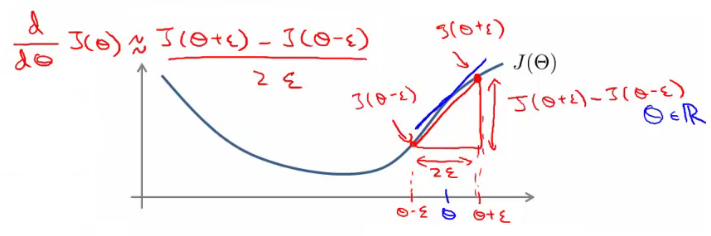
\includegraphics[width=\textwidth]{resources/gradient_checking}

\end{document}